\section{User Interface Storyboards}

\subsection{Administrative Functions: Kobe}
As an administrator, Kobe will need to approve or deny posts as needed and provide explanations for approval or denial (Figure \ref{fig:postmgmt}).  Before approval, Kobe will inspect each post to ensure that the posting follows the website's terms and conditions (Figure \ref{fig:postdetails}).  In addition, he will be able to contact and ban users, delete and edit user posts, and inspect user transaction history.  Priority 1 implementation shall be through MySQL workbench and/or MySQL command line interface.  The following user interface storyboards illustrate a priority 3 implementation for administration through the website.

\pagebreak
\begin{center}
\captionof{figure}{Post Management View}
\label{fig:postmgmt}
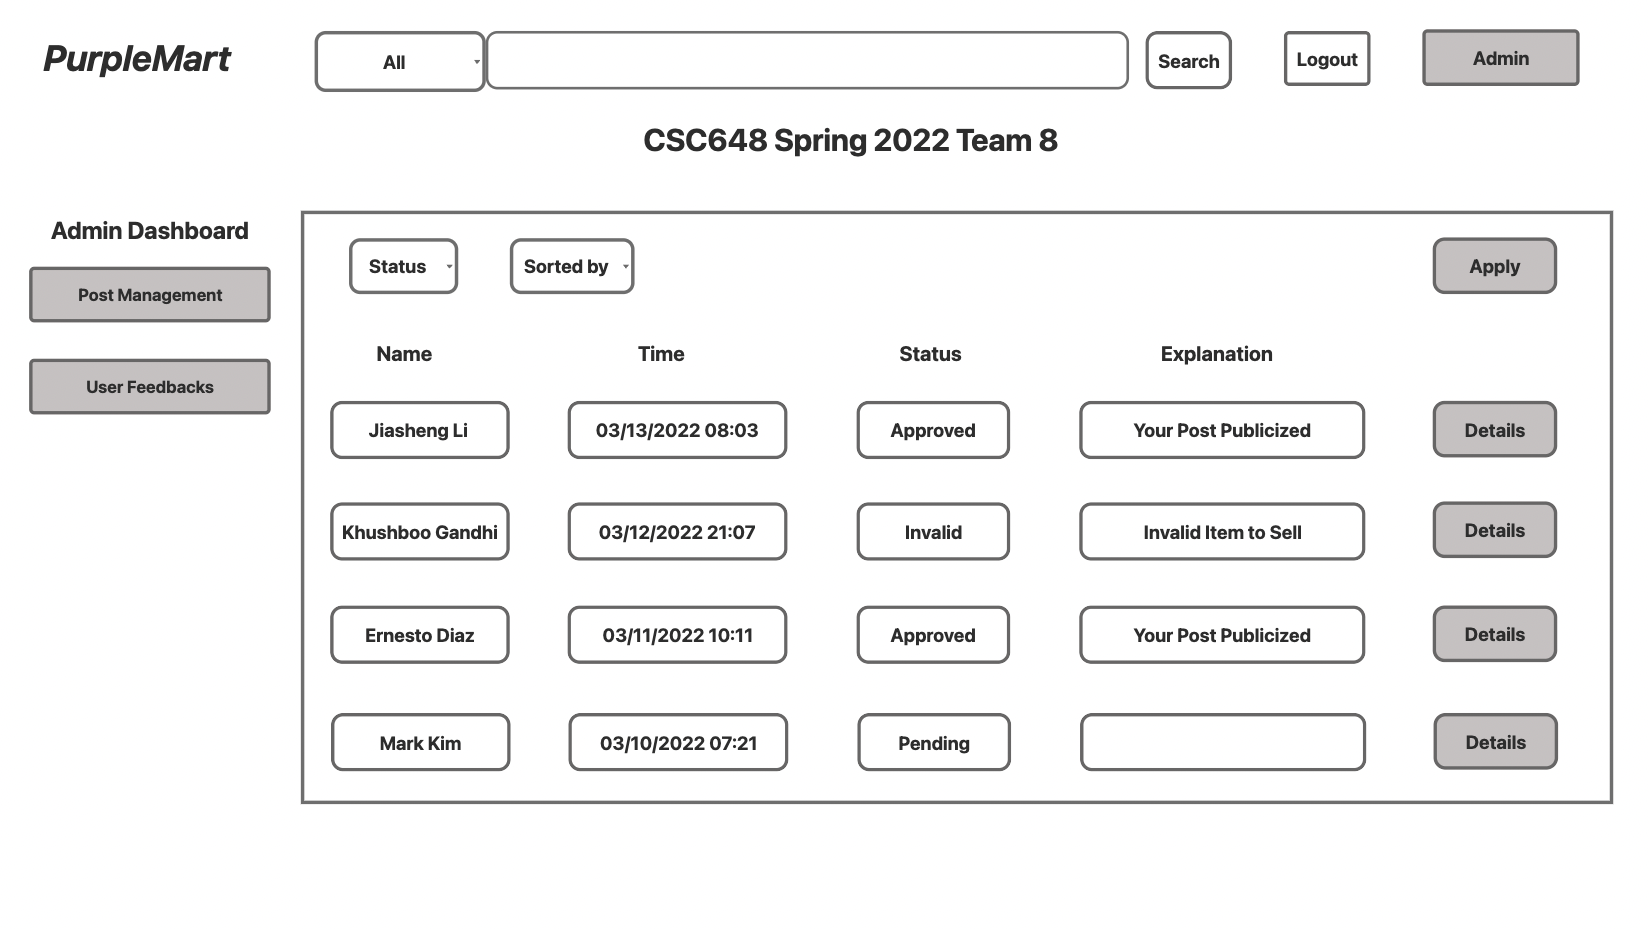
\includegraphics[trim={0 0 0 0}, width=\textwidth]{AdminDashboard_PostManagement}
\end{center}

\vspace{10mm}

\begin{center}
\captionof{figure}{Post Detail View}
\label{fig:postdetails}
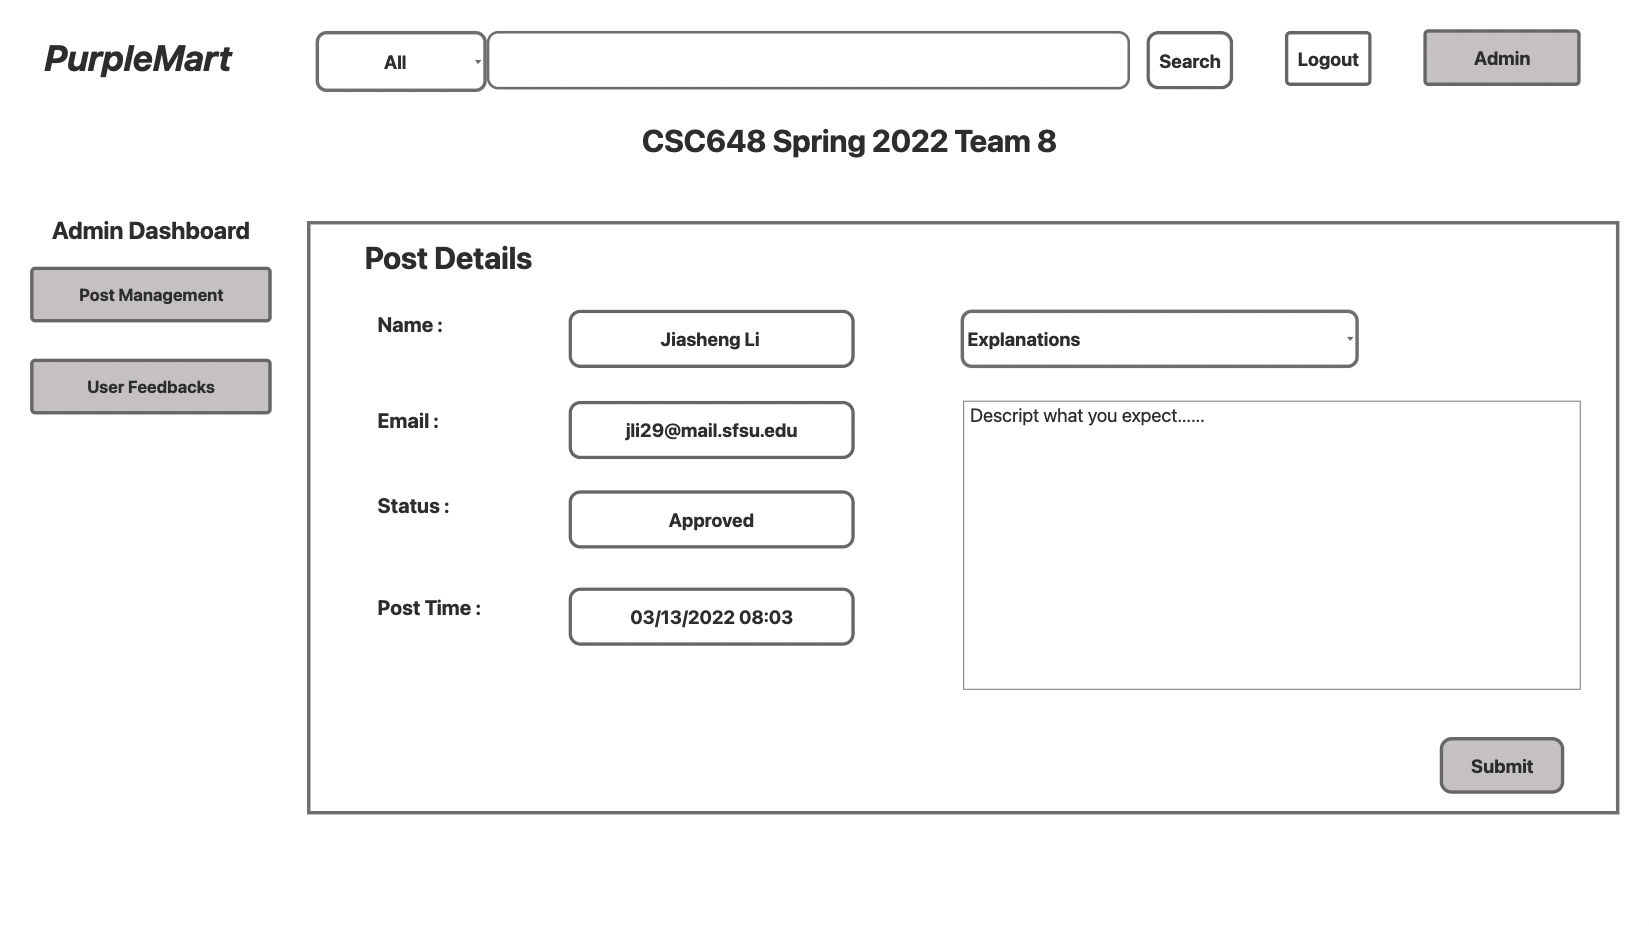
\includegraphics[trim={0 0 0 0}, width=\textwidth]{AdminDashboard_PostDetailEdit}
\end{center}

\pagebreak
\subsection{Purchase SFSU Apparel: Claire}
Claire is purchasing SFSU apparel from other users.  Using her laptop, she goes onto PurpleMarket and selects ``SFSU Apparel'' from the categories and browses the available listings (Figure \ref{fig:sfsu}).  Once she finds the swimsuit, she views the item details (Figure \ref{fig:itemc}), then attempts to message the seller for a swimsuit.  The website then informs her that to message a seller, she must first register for a free account or login (Figure \ref{fig:loginc}).  Since she is not signed up, she must register (Figure \ref{fig:regc}).  Once signed up, she is presented with a message page that allows her to message the seller (Figure \ref{fig:msgc}) and the website tells her that her message was successfully sent (Figure \ref{fig:msgconfc}).

\vspace{5mm}
\begin{center}
\captionof{figure}{SFSU Apparel Category Search}
\label{fig:sfsu}
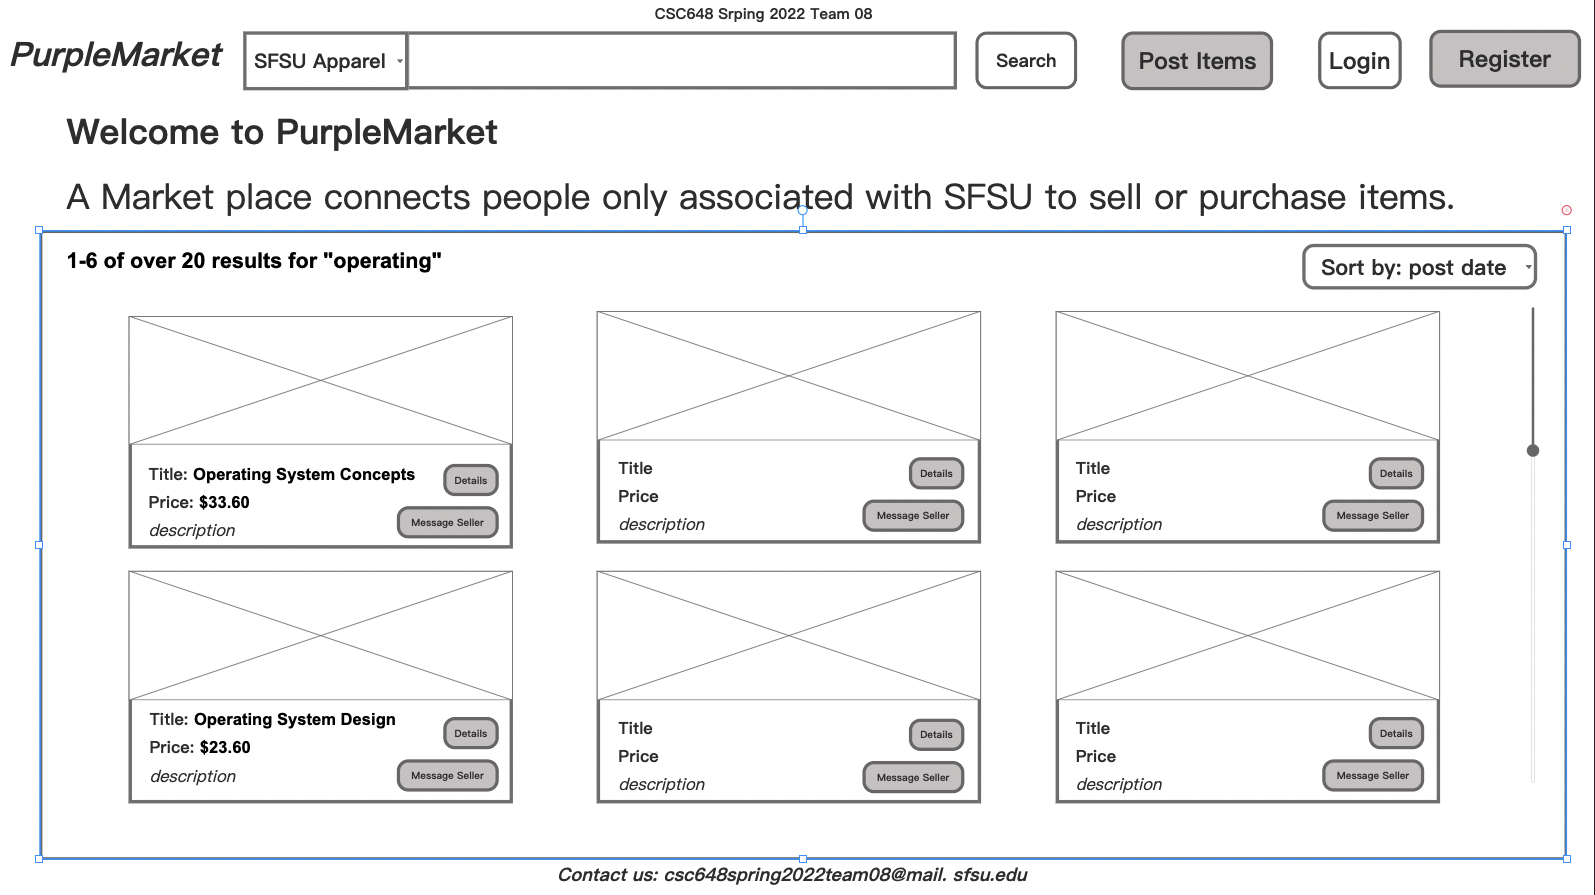
\includegraphics[trim={0 0 0 0}, width=\textwidth]{Search_SFSU}
\end{center}


\pagebreak

\begin{center}
\captionof{figure}{Item Detail View}
\label{fig:itemc}
\includegraphics[trim={0 -125 0 0}, width=\textwidth]{item}
\end{center}

\begin{center}
\captionof{figure}{Login View}
\label{fig:loginc}
\includegraphics[trim={0 0 0 0}, width=\textwidth]{login}
\end{center}

\pagebreak

\begin{center}
\captionof{figure}{Registration View}
\label{fig:regc}
\includegraphics[trim={0 -125 0 0}, width=\textwidth]{registration}
\end{center}

\begin{center}
\captionof{figure}{Message View}
\label{fig:msgc}
\includegraphics[trim={0 0 0 0}, width=\textwidth]{message}
\end{center}

\pagebreak

\begin{center}
\captionof{figure}{Message Confirmation View}
\label{fig:msgconfc}
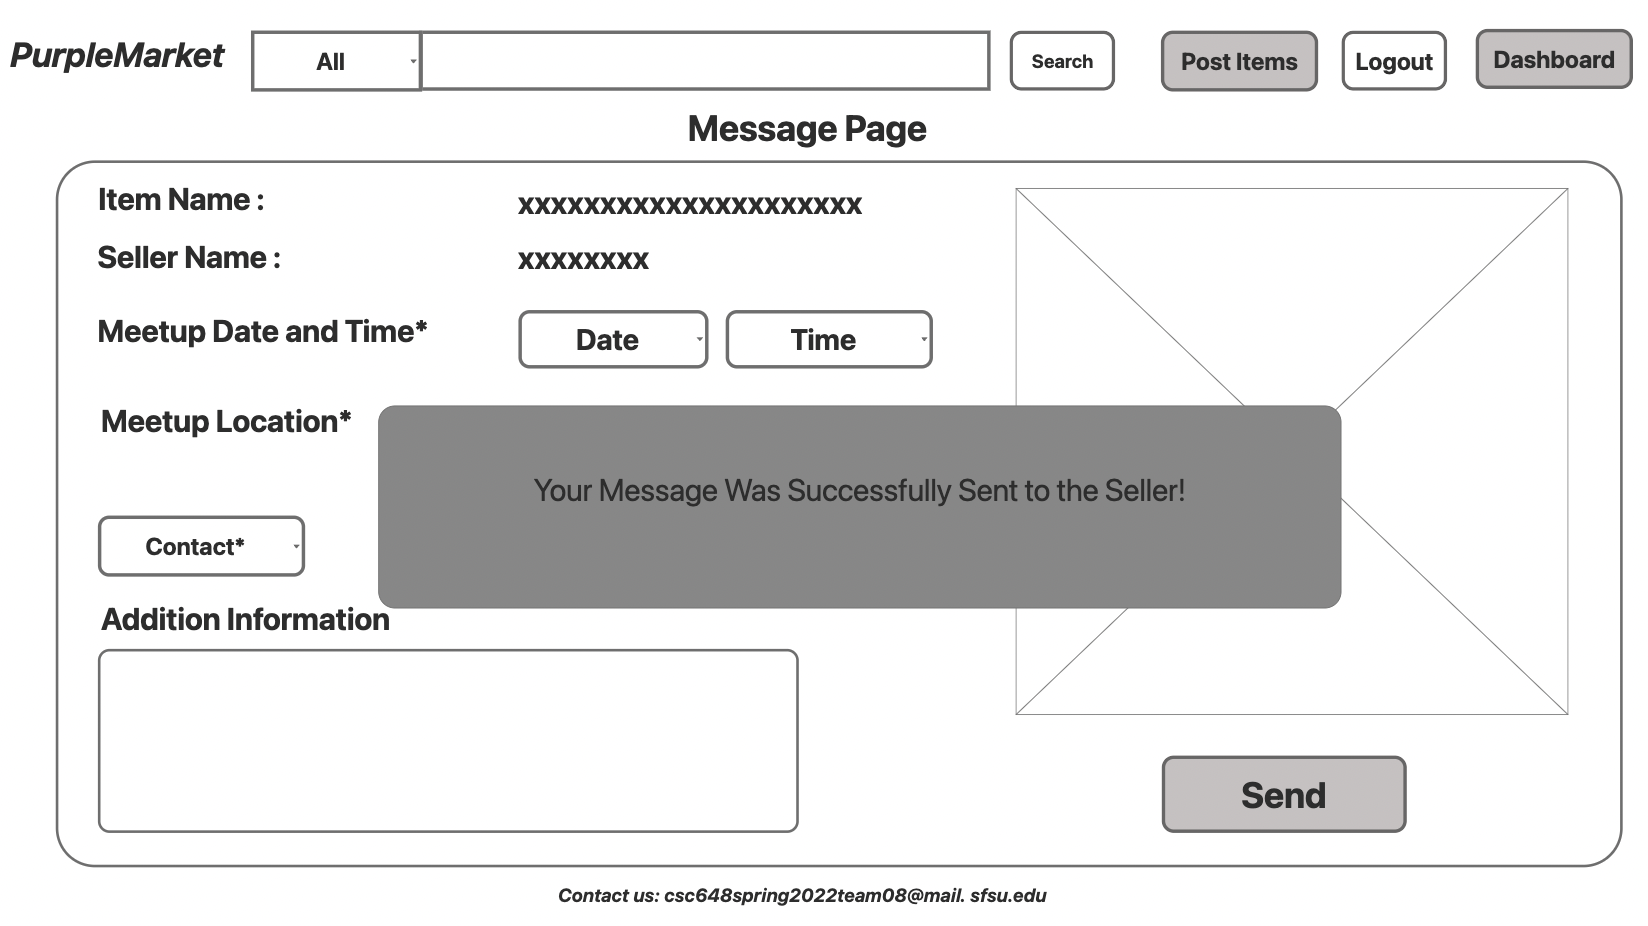
\includegraphics[trim={0 0 0 0}, width=\textwidth]{Message_Confirmation}
\end{center}

\subsection{Request Items: Anna}
Anna wants to get a copy of notes from her class from a previous student of hers.  She goes to PurpleMarket to search for notes from her course (Figure \ref{fig:notes}).  After finding a student posting some notes that he took from Anna's class last semester (Figure \ref{fig:itema}), Anna messages him to get a copy.  When she attempts to contact him, the website prompts her to login or register (Figure \ref{fig:logina}).  Since she is already registered, she logs in and messages the student to set up a meeting on campus (Figures \ref{fig:msga}, \ref{fig:msgconfa}).

\pagebreak

\vspace{5mm}
\begin{center}
\captionof{figure}{Search for Notes}
\label{fig:notes}
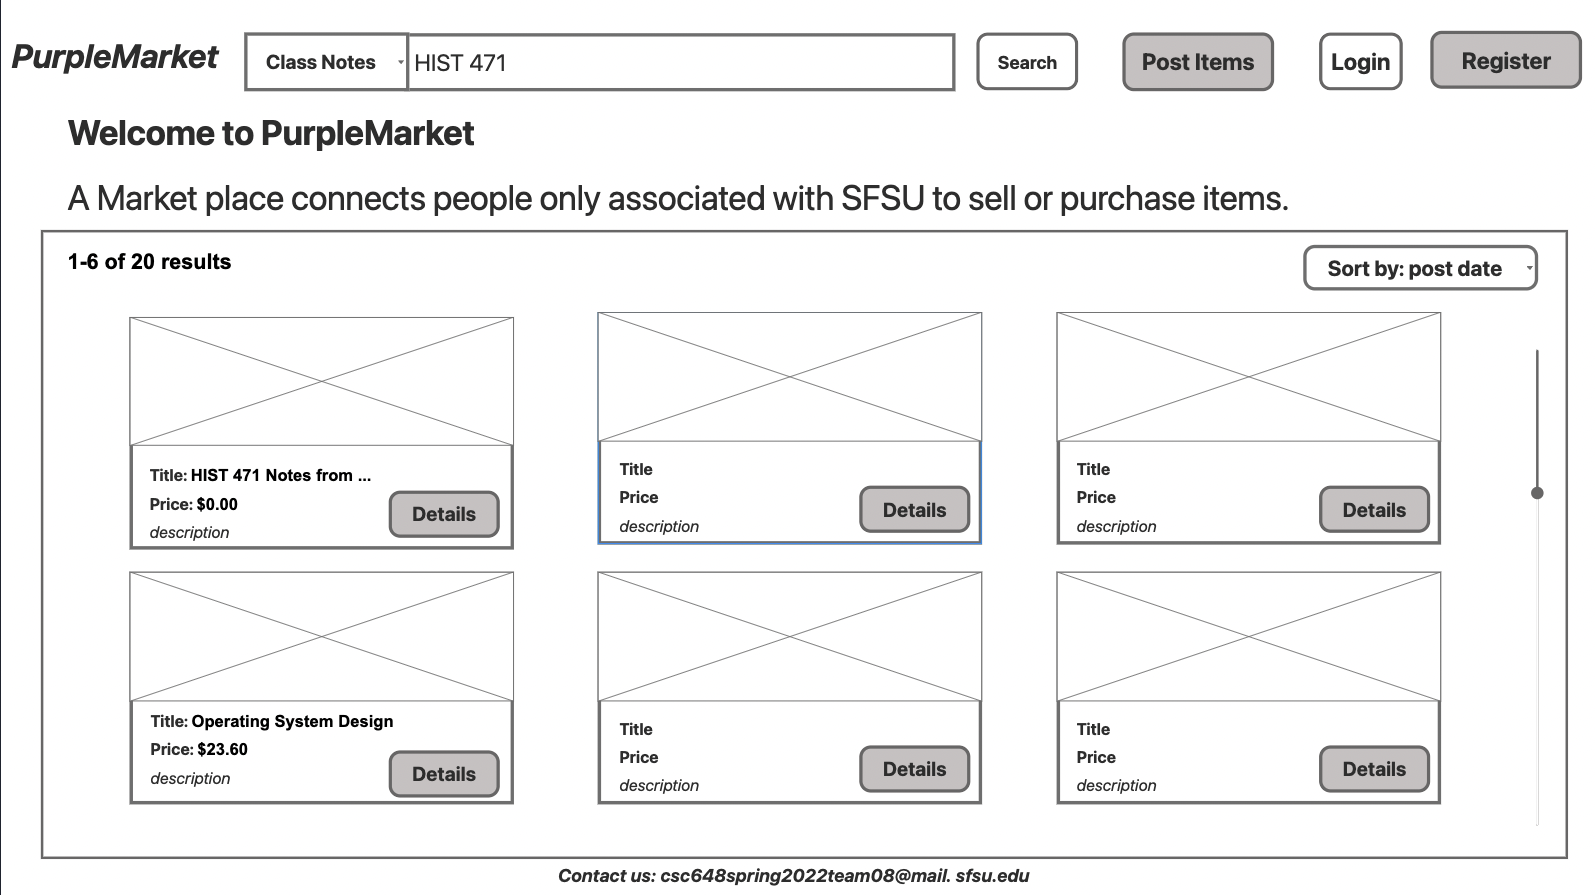
\includegraphics[trim={0 0 0 0}, width=\textwidth]{hist}
\end{center}

\begin{center}
\captionof{figure}{Item Detail View}
\label{fig:itema}
\includegraphics[trim={0 -125 0 0}, width=\textwidth]{item}
\end{center}

\pagebreak

\begin{center}
\captionof{figure}{Login View}
\label{fig:logina}
\includegraphics[trim={0 0 0 0}, width=\textwidth]{login}
\end{center}

\begin{center}
\captionof{figure}{Message View}
\label{fig:msga}
\includegraphics[trim={0 0 0 0}, width=\textwidth]{message}
\end{center}

\pagebreak

\begin{center}
\captionof{figure}{Message Confirmation View}
\label{fig:msgconfa}
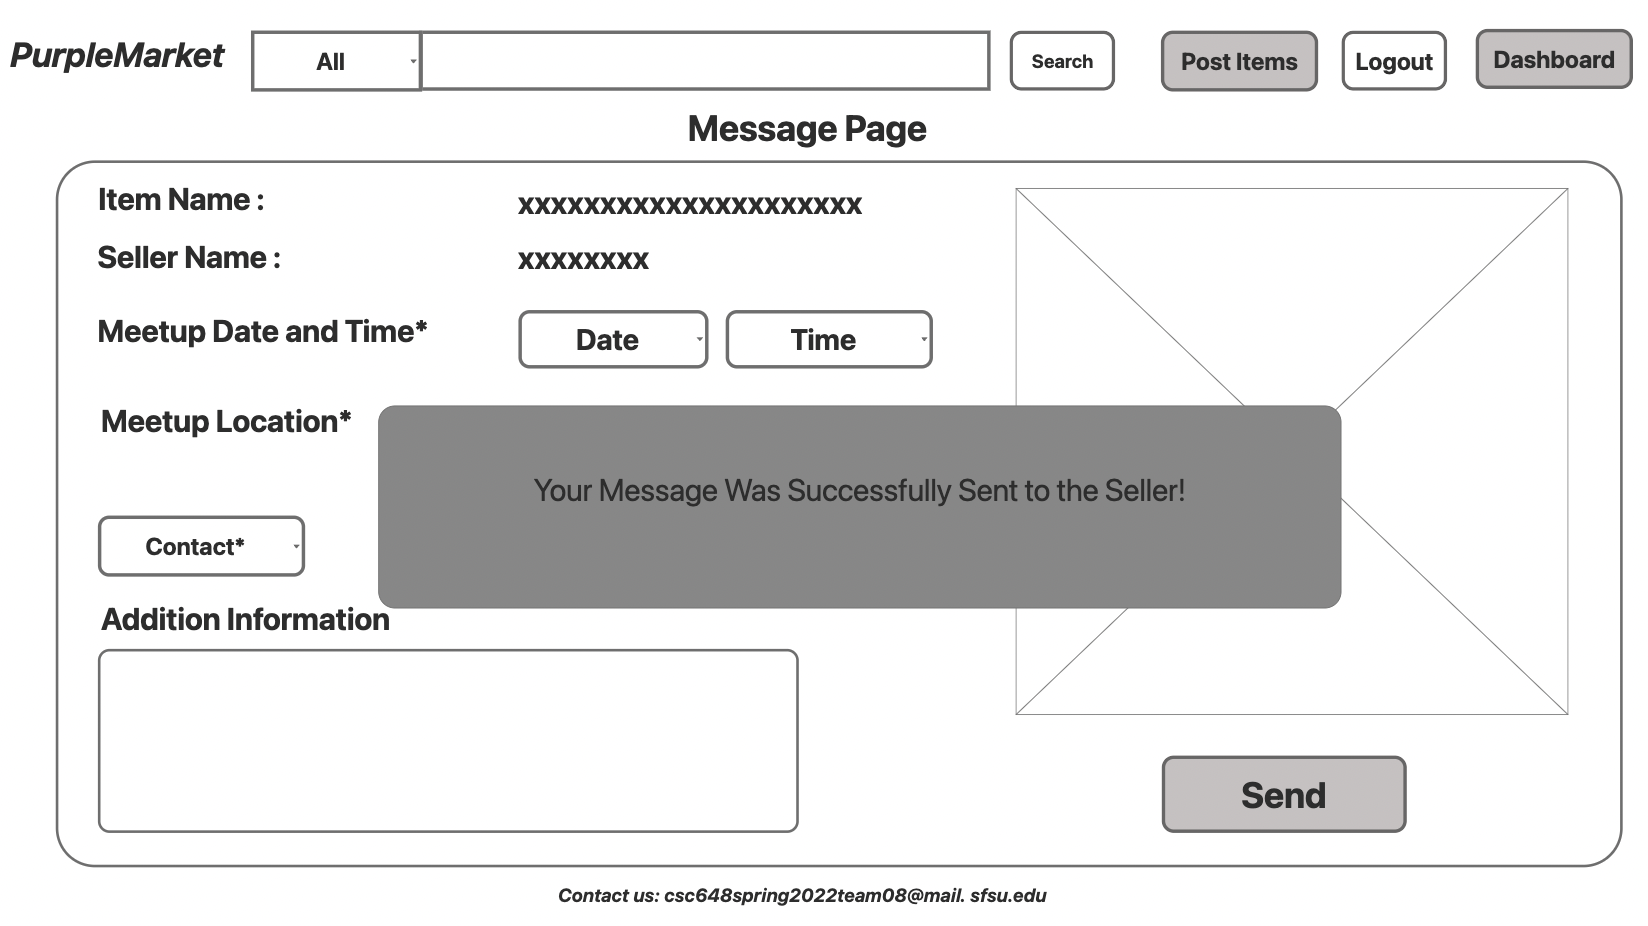
\includegraphics[trim={0 0 0 0}, width=\textwidth]{Message_Confirmation}
\end{center}

\subsection{Browsing for Items: Curry}
Curry is just curious about what used items he can score on PurpleMarket, so he visits the website to browse around.  While browsing, he remembers that there is a book he's been wanting to read.  He does a search on the page for the book title that he's looking for (Figure \ref{fig:book}). He checks the details of the item post to make sure it is exactly what he wants (Figure \ref{fig:itemy}).  As a long-time website user, he is already logged in, so he immediately messages the user to set up a time and location for the purchase (Figures \ref{fig:msgy}, \ref{fig:msgconfy}).

\pagebreak

\vspace{5mm}
\begin{center}
\captionof{figure}{Search for a Book}
\label{fig:book}
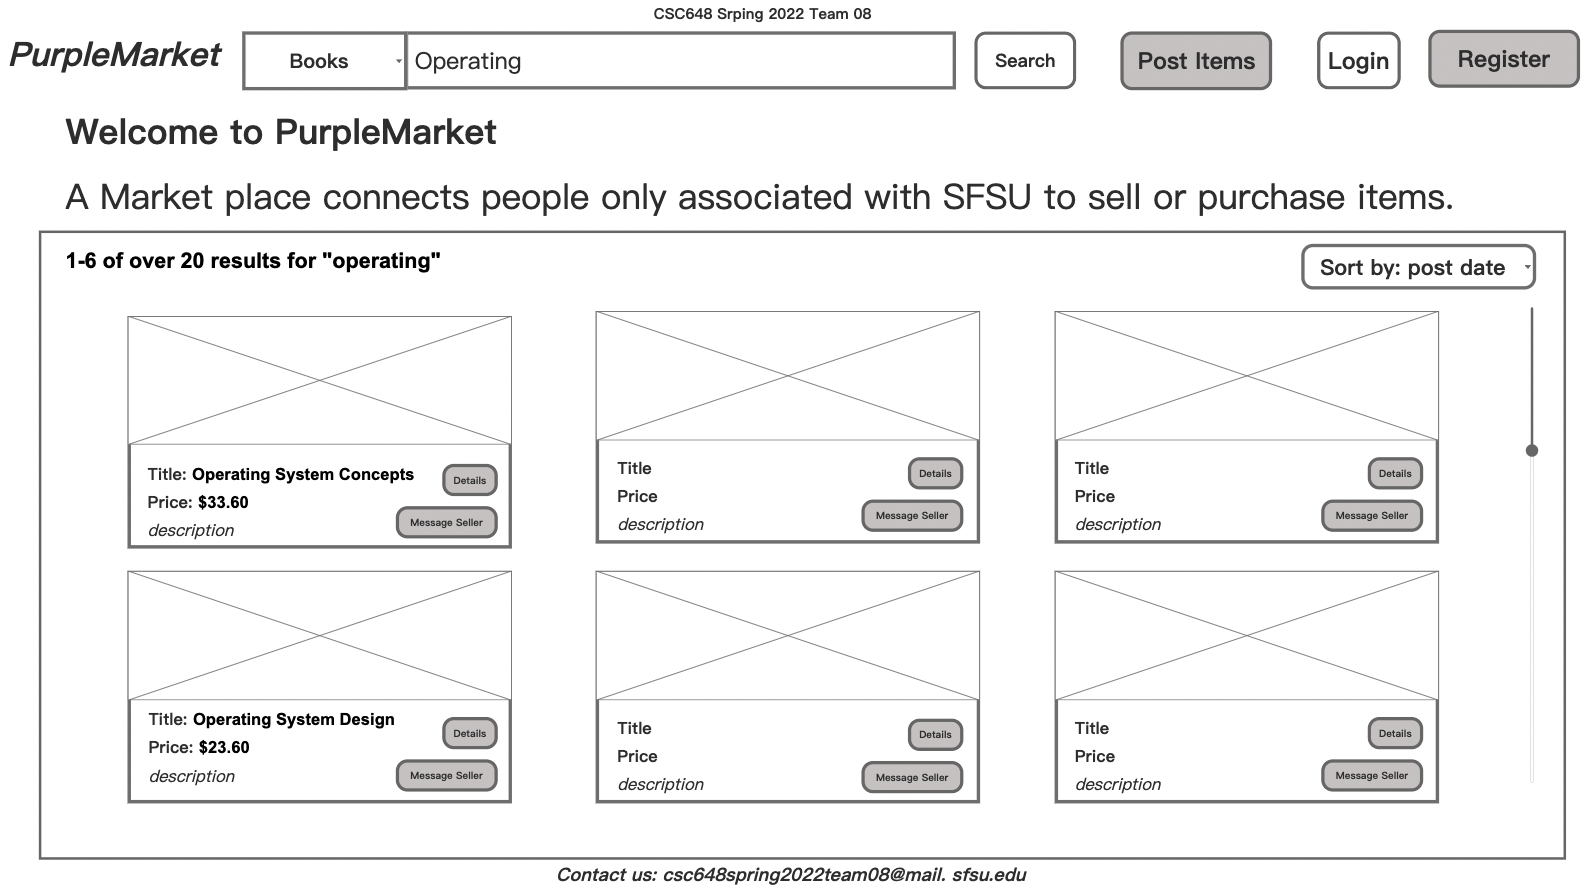
\includegraphics[trim={0 0 0 0}, width=\textwidth]{book}
\end{center}

\begin{center}
\captionof{figure}{Item Detail View}
\label{fig:itemy}
\includegraphics[trim={0 -125 0 0}, width=\textwidth]{item}
\end{center}

\pagebreak

\begin{center}
\captionof{figure}{Message View}
\label{fig:msgy}
\includegraphics[trim={0 0 0 0}, width=\textwidth]{message}
\end{center}

\begin{center}
\captionof{figure}{Message Confirmation View}
\label{fig:msgconfy}
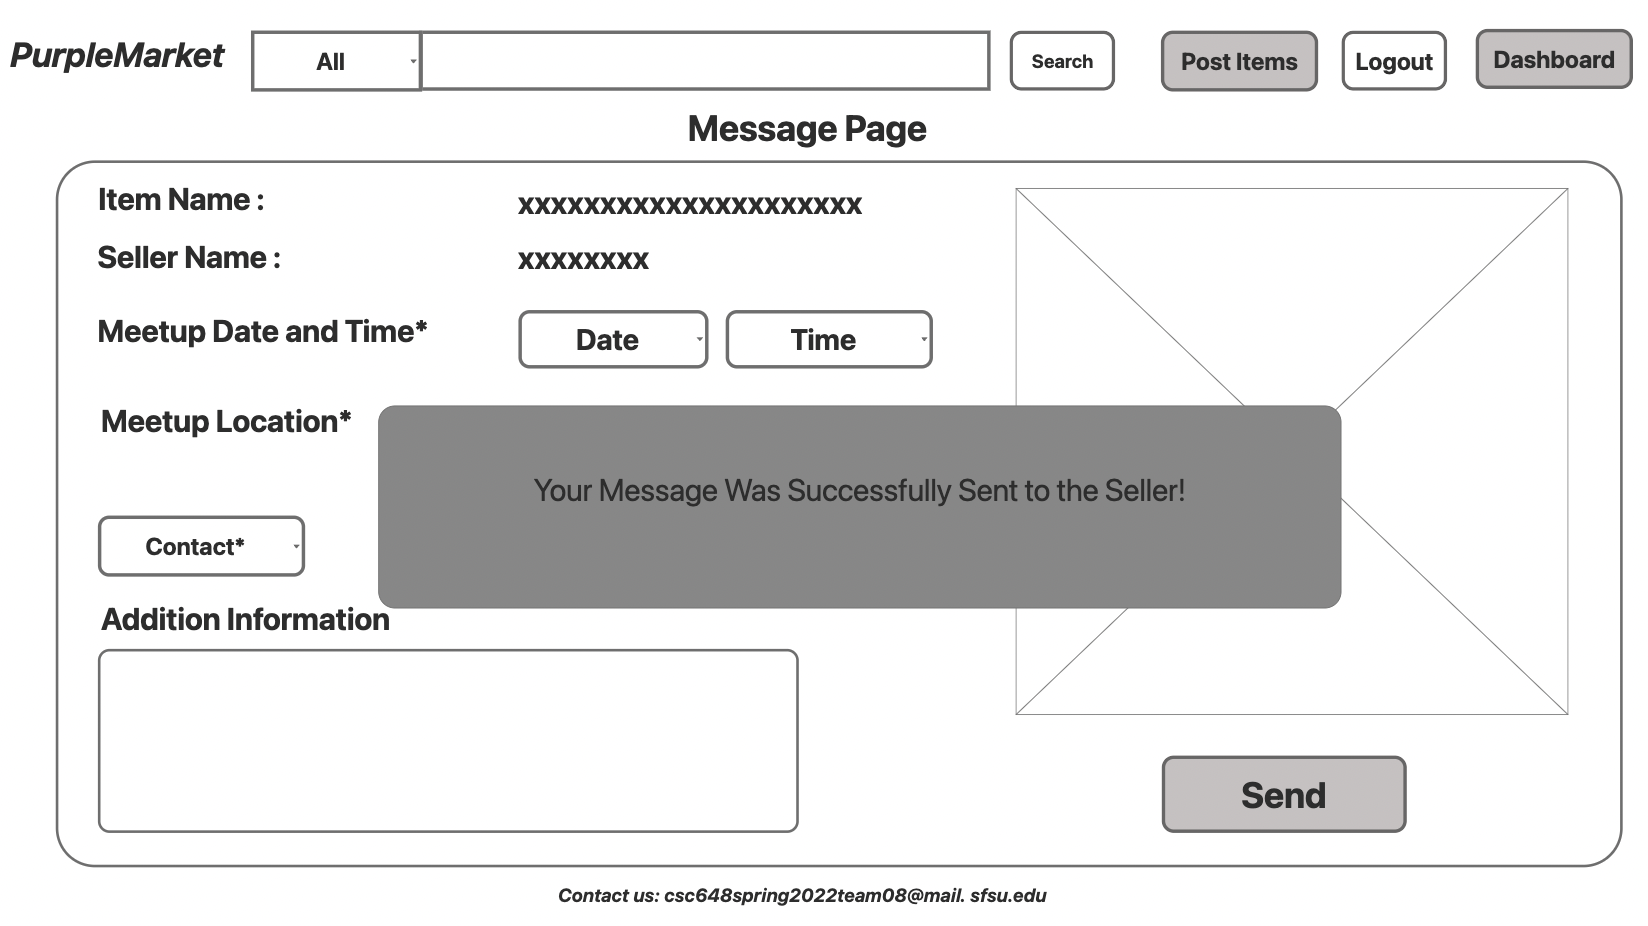
\includegraphics[trim={0 0 0 0}, width=\textwidth]{Message_Confirmation}
\end{center}

\subsection{Selling Furniture: Anna}
Anna has a bookshelf to sell, so she visits PurpleMarket to list the item.  From the main homepage, she easily finds the button to post her item for sale (Figure \ref{fig:home}).  Once on the post page (Figure \ref{fig:postitema}), she enters the details of her bookshelf and uploads a photo.  When she attempts to post, the site requests that she log in (Figure \ref{fig:loginb}).  Once logged in, she can post her item.  The website tells her that she will need to wait about 24 hrs for her post to be approved and go live (Figure \ref{fig:postconfb}).  She receives a message when it is approved and published.  She goes to her dashboard to look at the approval message (Figure \ref{fig:dashb}).

\vspace{5mm}
\begin{center}
\captionof{figure}{Main Homepage}
\label{fig:home}
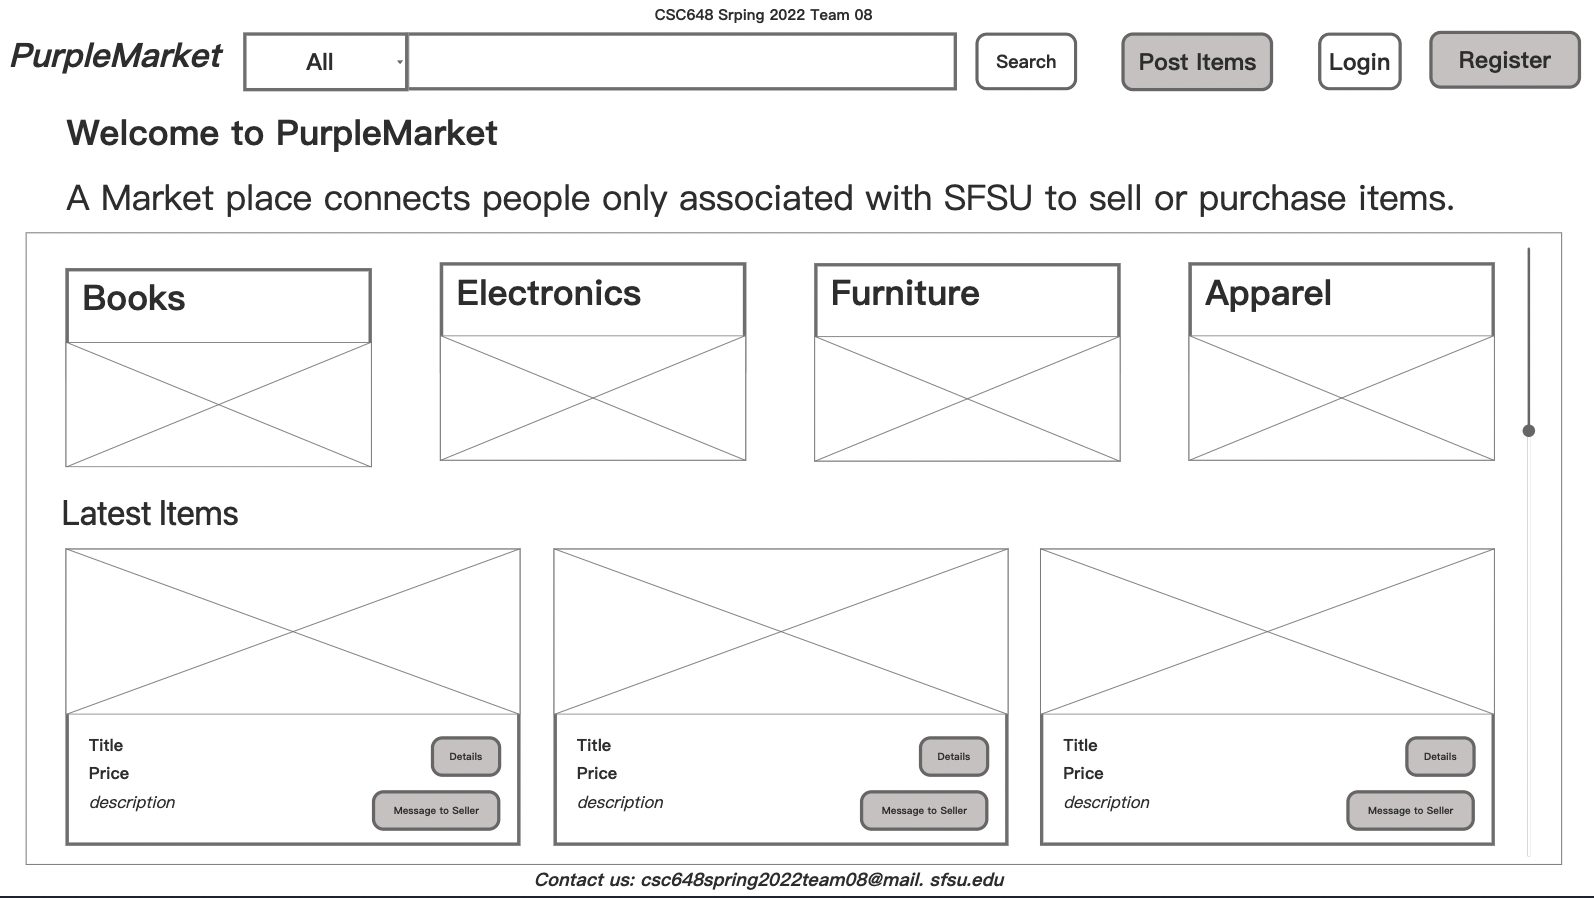
\includegraphics[trim={0 0 0 0}, width=\textwidth]{Home_Anonymous}
\end{center}

\pagebreak

\begin{center}
\captionof{figure}{Post Item View}
\label{fig:postitema}
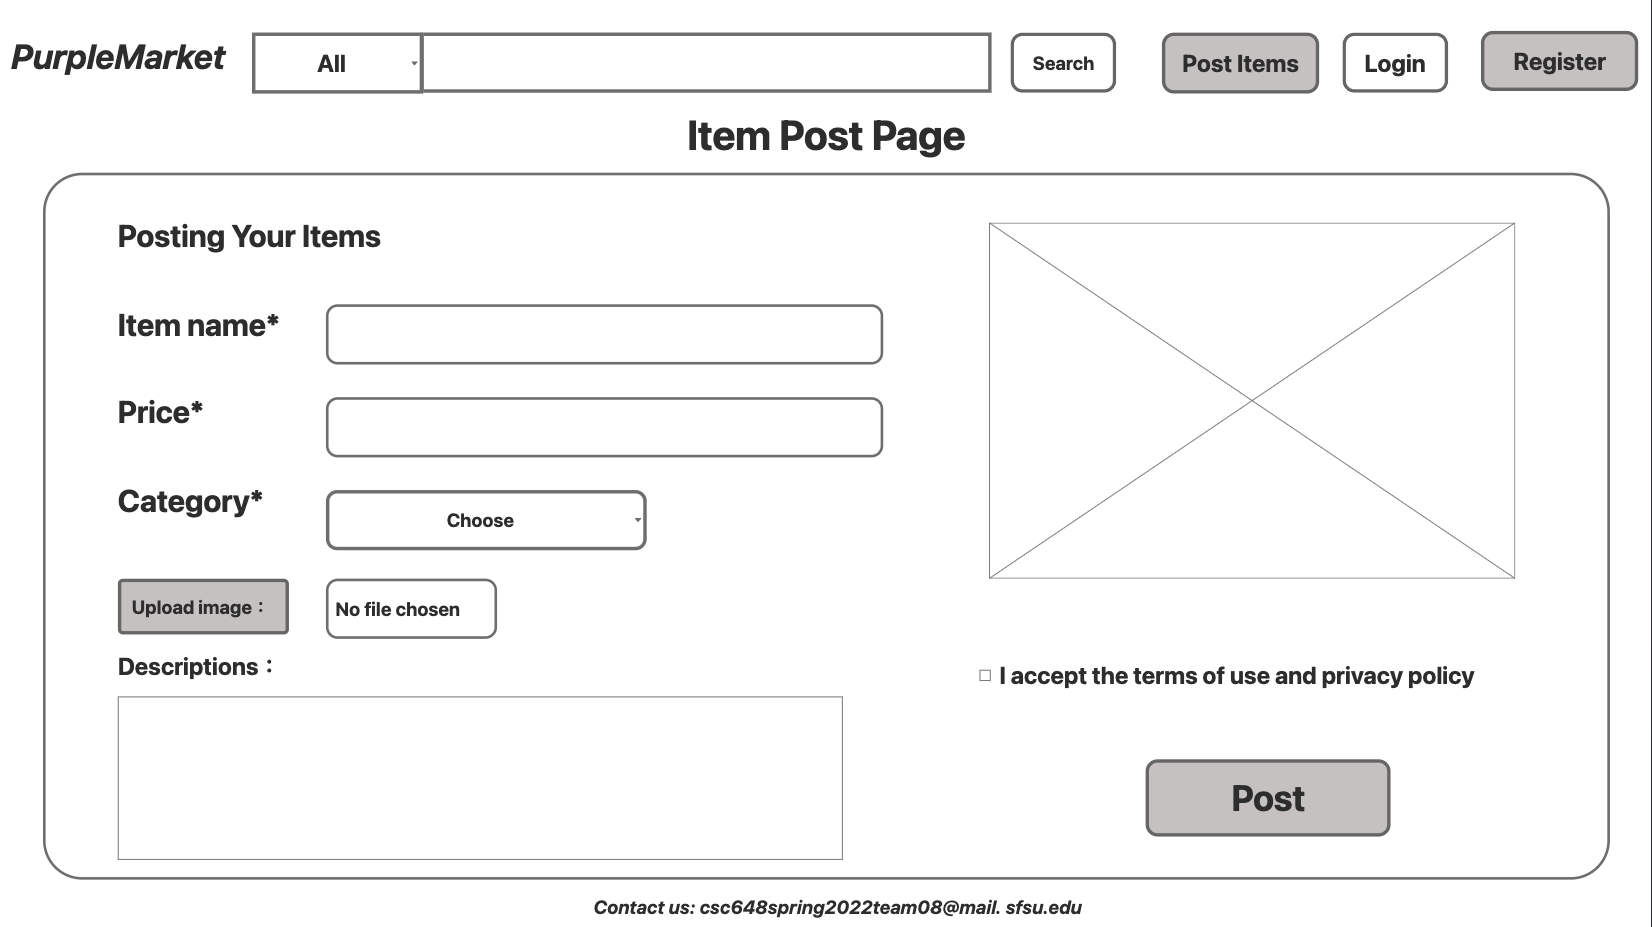
\includegraphics[trim={0 -125 0 0}, width=\textwidth]{PostItem}
\end{center}

\begin{center}
\captionof{figure}{Login View}
\label{fig:loginb}
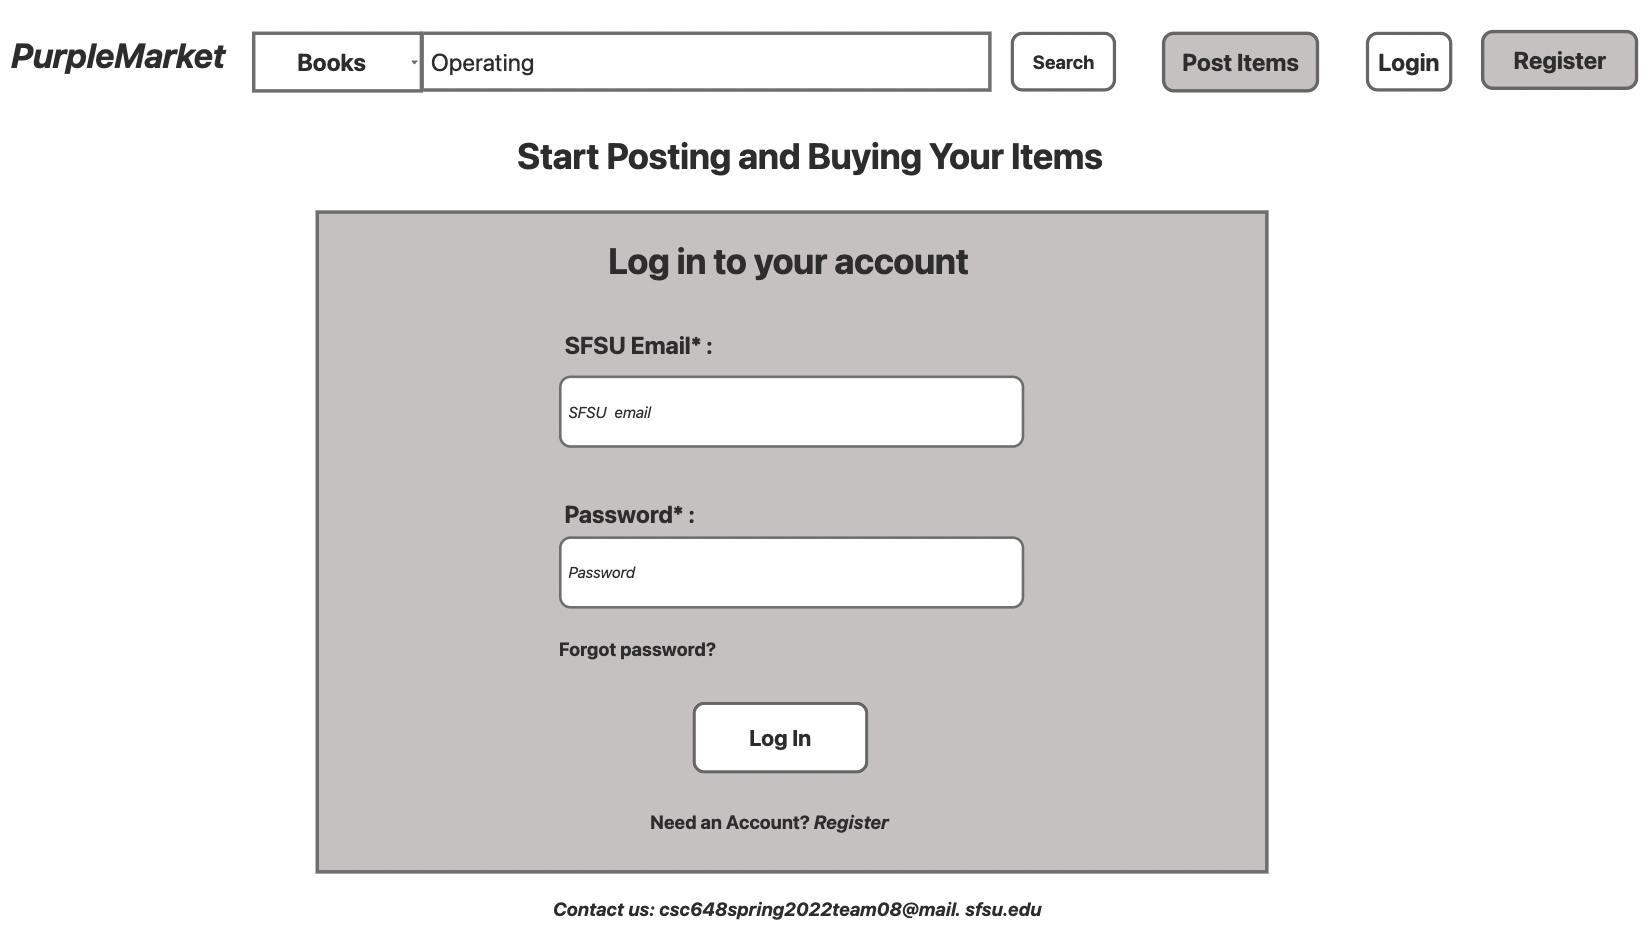
\includegraphics[trim={0 0 0 0}, width=\textwidth]{Login}
\end{center}

\pagebreak

\begin{center}
\captionof{figure}{Message Confirmation View}
\label{fig:postconfb}
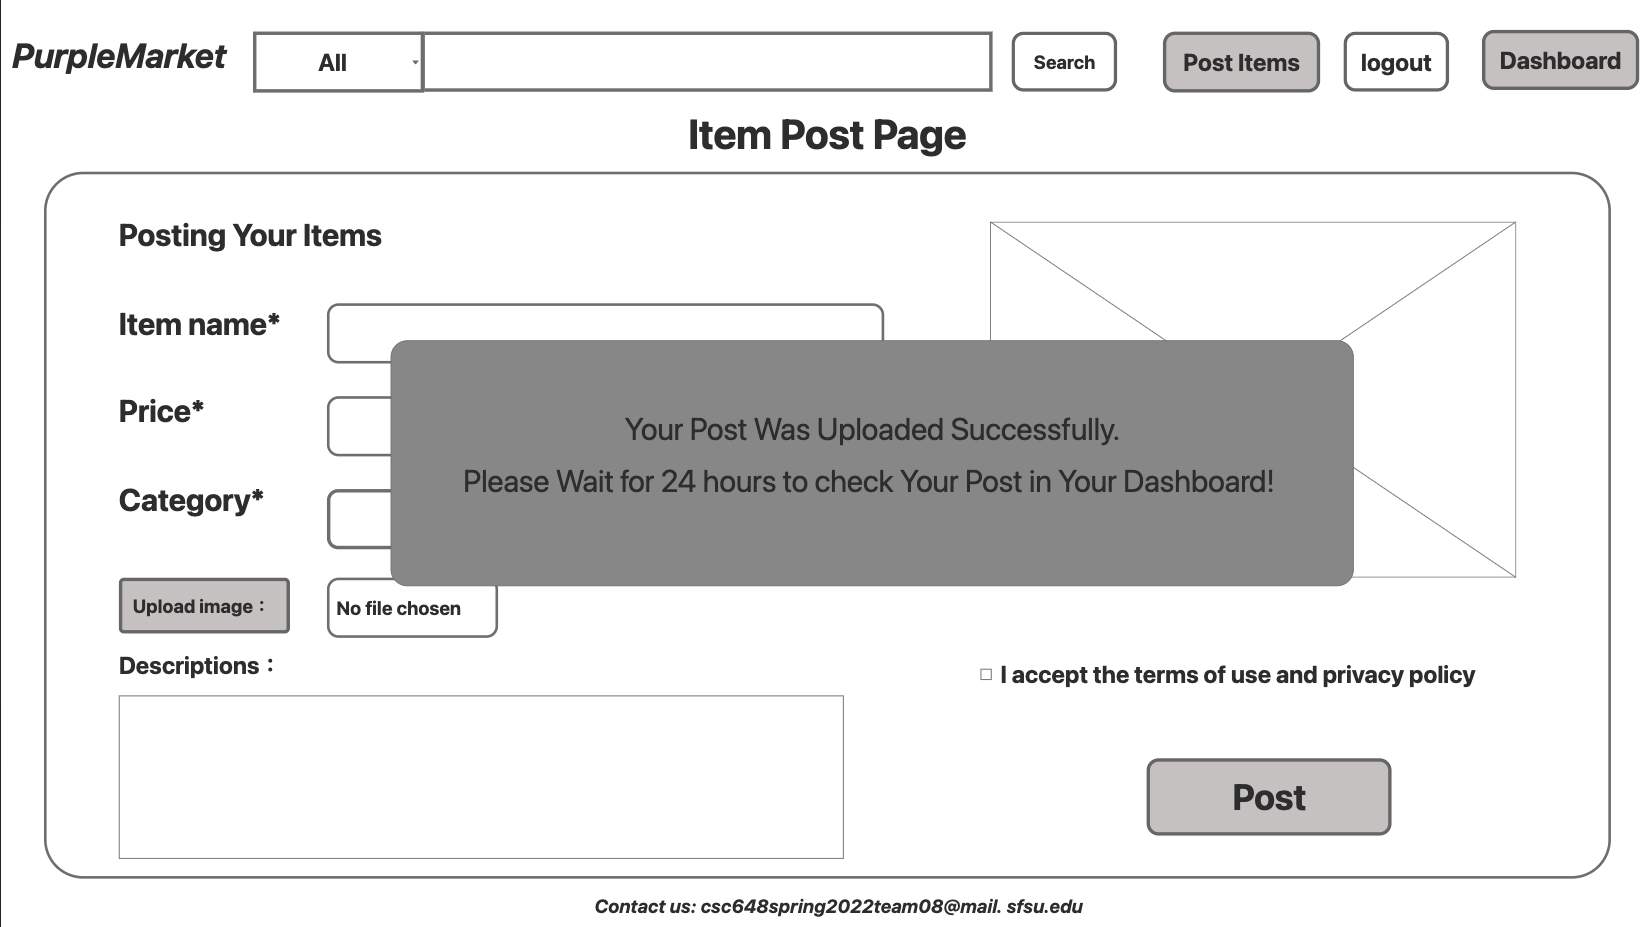
\includegraphics[trim={0 0 0 0}, width=\textwidth]{PostItem_Confirmation}
\end{center}

\begin{center}
\captionof{figure}{User Dashboard}
\label{fig:dashb}
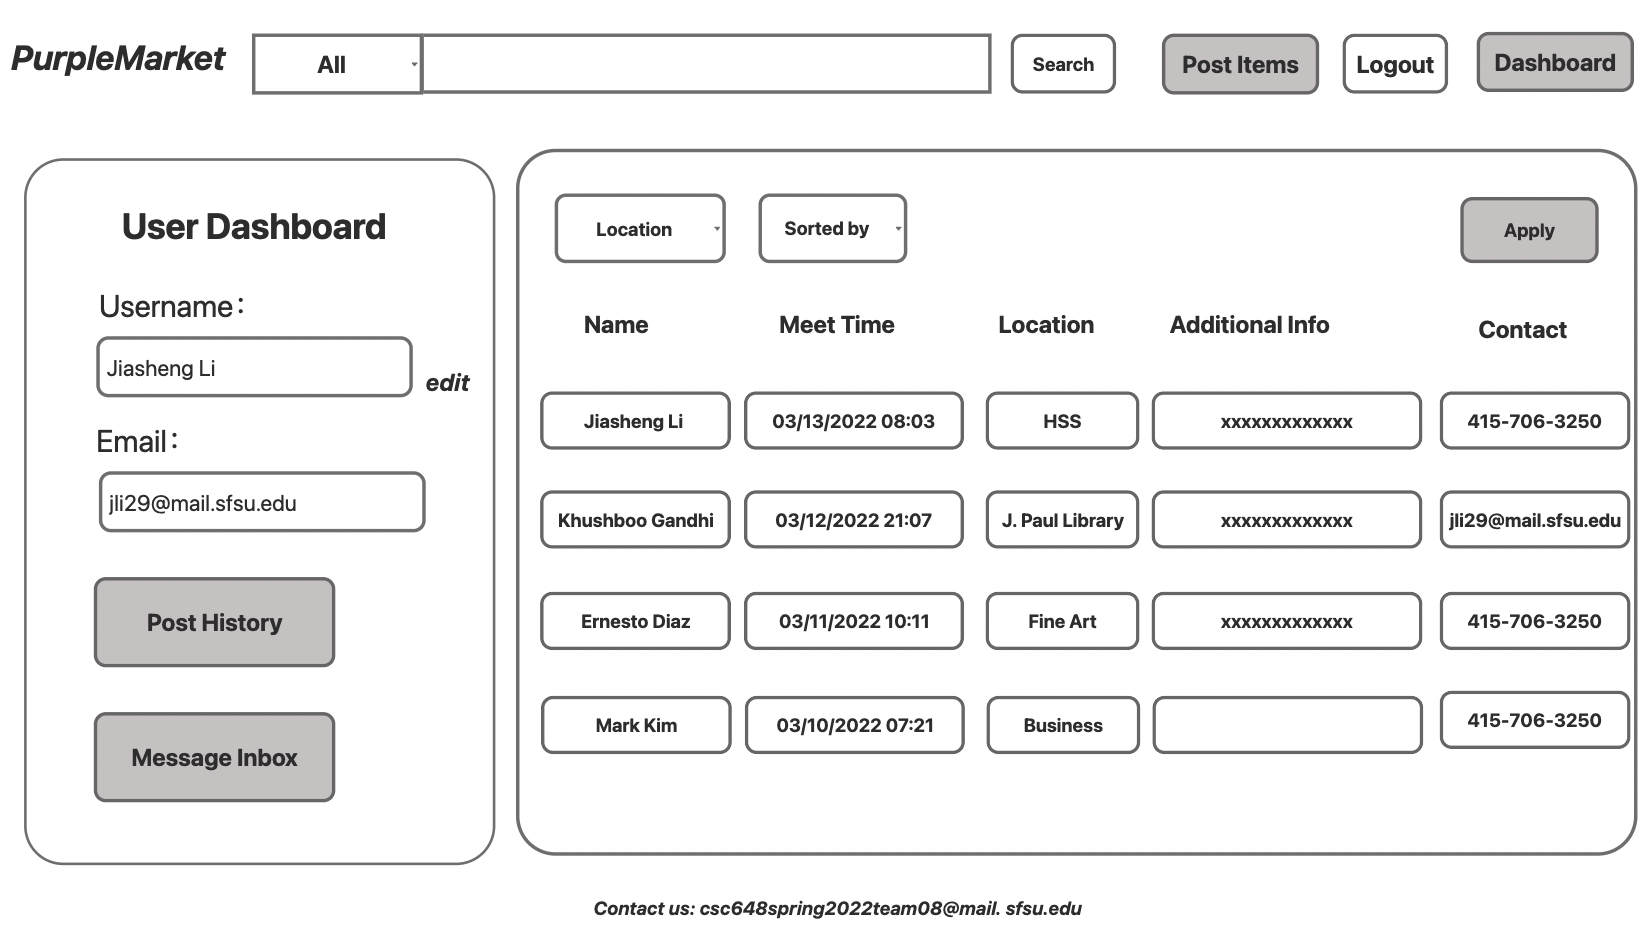
\includegraphics[trim={0 0 0 0}, width=\textwidth]{UserDashboard_MessageHistory}
\end{center}

